\section{Model optimization and sensitivity analysis}
\subsection{Add new starting point or delete existing point.}
DNA evidence \parencite{pestfr} showed that the hornets in Washington and Vancouver were unrelated and came from different nests \parencite{attachment}, which suggests that there is more than one pest invasion time and place. Therefore, for our spread model, it may have multiple starting points. In addition, the government's vigorous crackdown method is to directly destroy the Hornet's nest, which will have a greater impact on our simulation results. Therefore, after every nest destruction, our simulation model also needs to be adjusted accordingly.

When new reports are given over time, we may encounter a problem that some verified hornet locations is outside of our simulated area. Regarding how to determine that this new pest emergence point is a new invasion point, we have the following update mechanism.
\begin{itemize}
    \item In these extracted reports, we find the most earliest one due to its detection time.
    \item Then we add a new starting point at this place on its detection date and set the initial population as 200.
    \item We run the PS-CA model again from the first day and we repeat the above steps until all the given positive reports are included in our simulation region.
\end{itemize}

By contrast, the government has taken actions to interfere with the pest spread. When an existing nest is destroyed, we clear the state number of the place in our cellular automata model immediately.

%%插图 标点精确度分析
\begin{figure}[H] 
\begin{minipage}[t]{0.5\linewidth} 
\centering 
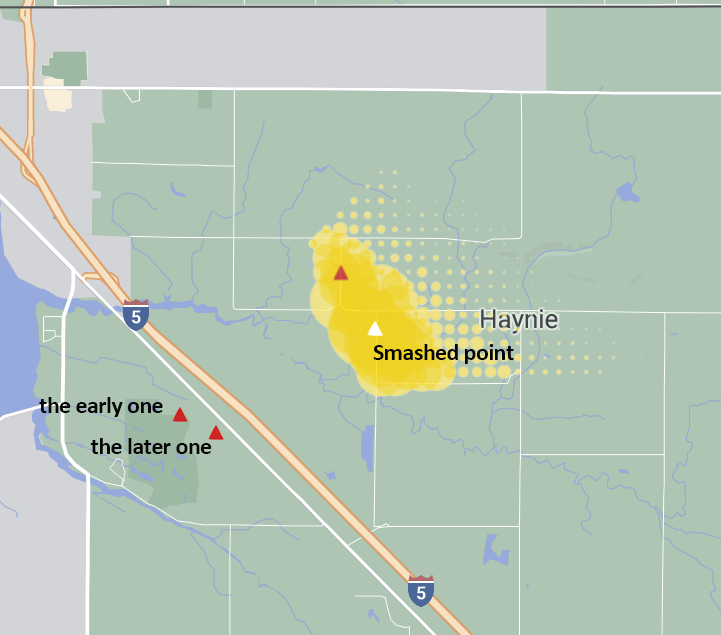
\includegraphics[width=2.5in]{Chapter-2021C/images-2021C/4-before.png} 
\caption{Before update.} 
\label{fig:2021C-4Before update.} 
\end{minipage}
\begin{minipage}[t]{0.5\linewidth} 
\centering 
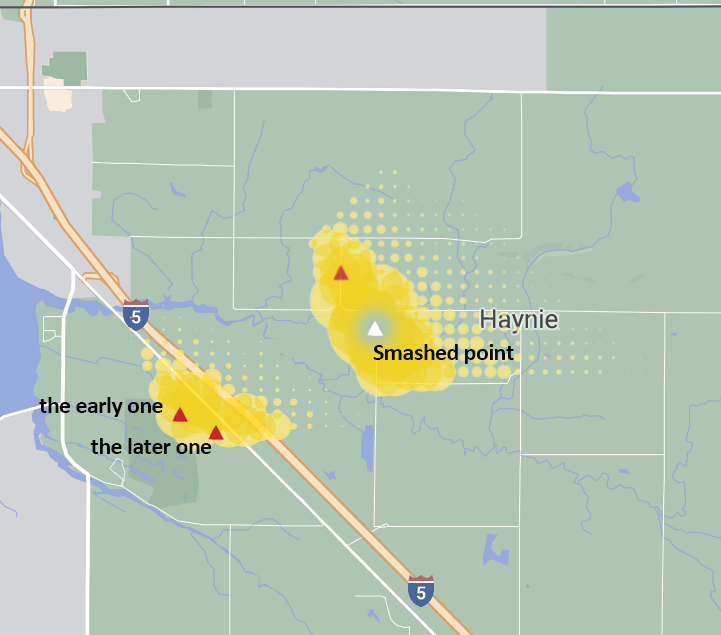
\includegraphics[width=2.5in]{Chapter-2021C/images-2021C/4-after.png} 
\caption{After update.} 
\label{fig:2021C-4After update.} 
\end{minipage} 
\end{figure}

The former Figure \ref{fig:2021C-4Before update.} and \ref{fig:2021C-4After update.} is an example of our update rule. The picture on the right vividly shows how we add a new starting point and delete an existing point.

Due to the uncertainty of the time of pest invasion and destruction, we must update the simulation mechanism every time we receive a nest change.

\subsection{Adjust Pest Growth Curve}
Initially, we ignore the impact of human intervention and environmental capacity on the growth and reproduction of pest, so we set its growth curve as a J-type growth. And now, due to the government's destruction of pest nests, we should consider this impact.

It is known from the literature that the annual population loss of bees is about 9.5-10.7\% \parencite{Chinesebee}. This is almost the same for Vespa mandarinia  in the same suborder as bees. As for human intervention factors, we can't get a precise impact number, so we might as well assume that the population of pests is decreasing year by year, that is change $\lambda$ from 1.2 to 0.8. 
As for the update frequency, we recommend that it be adjusted once a year based on the government's prevention and control efforts.

\subsection{Eradication Evidence Constitution and Sensitivity analysis}

To investigate whether or not the pest has been eradicated in Washington State, we define an index $Degree_{eradication}$ for the degree of eradication. The index is calculated by the quotient of the total number at $t$ time and the initial number. We set three limits to the index as to show the degree of eradication. More thorough eradication implies smaller index.

\begin{equation*}
    \label{eq:degree}
    Degree_{eradication} = \frac{\sum^n_{i=1} p_{i,t}}{p_{start,1}} \begin{cases}
    <1, & \text{under control but still need more intervention}; \\
    <0.1, & \text{effective but still need more observation}; \\
    <0.01, & \text{thorough eradication}.
    \end{cases}
\end{equation*}

Based on the degree of eradication, we run the cellular automata model to calculate the intervention period until the degree satisfy the criteria. In addition, we make sensitivity analysis towards the intervention period related to $\lambda$.

%%插图 sensitivity analysis
\begin{figure}[H] 
\begin{minipage}[t]{0.5\linewidth} 
\centering 
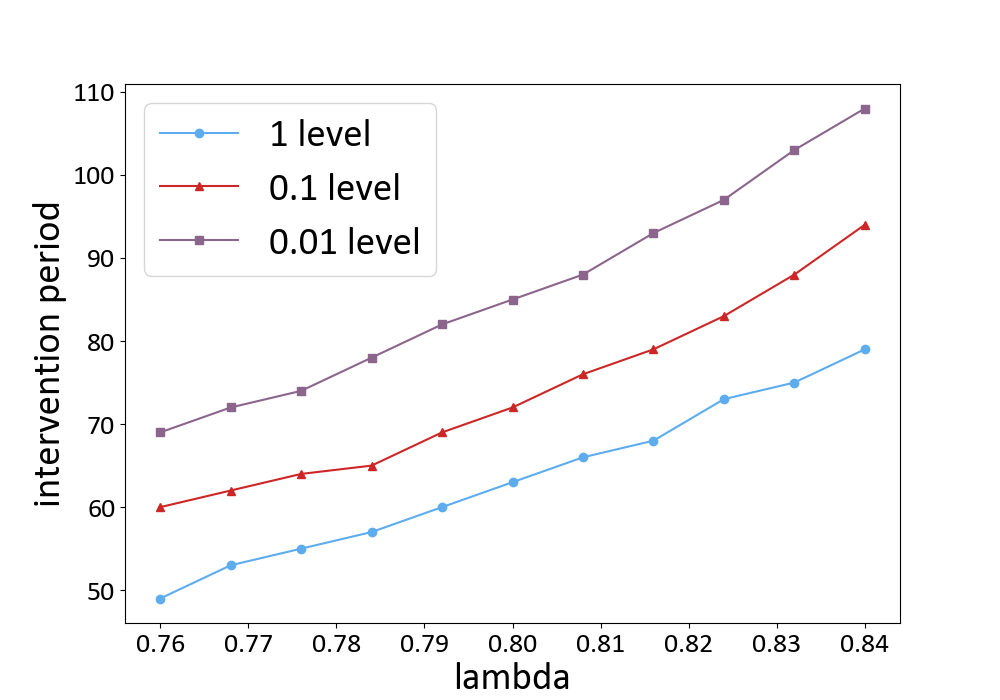
\includegraphics[width=3in]{Chapter-2021C/images-2021C/4-sensitivity.png} 
\caption{Intervention period.} 
\label{fig:2021C-Intervention period.} 
\end{minipage}
\begin{minipage}[t]{0.5\linewidth} 
\centering 
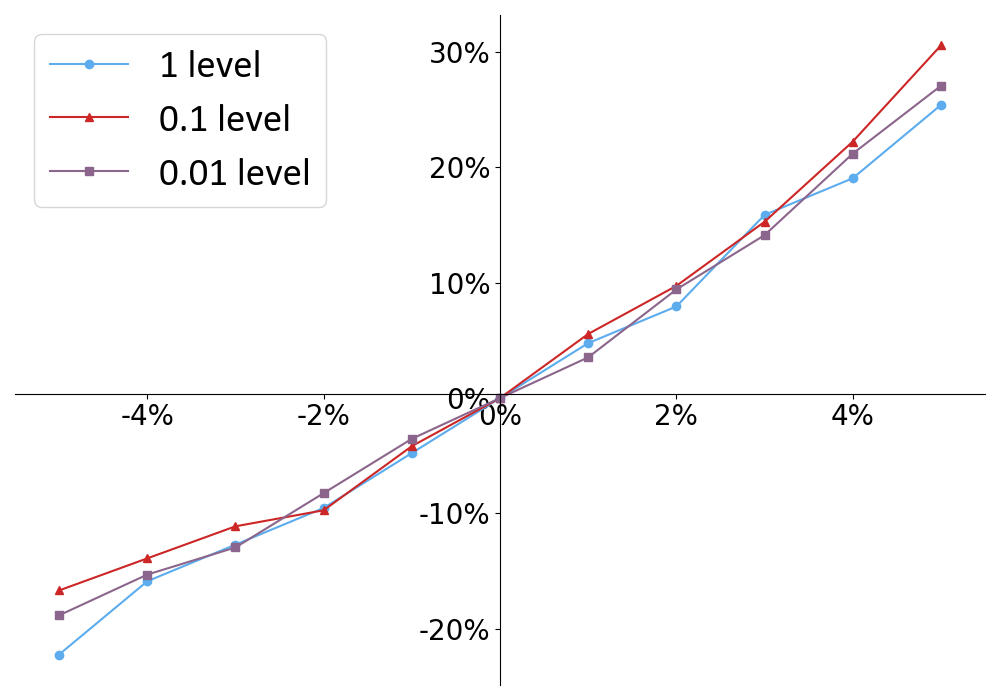
\includegraphics[width=3in]{Chapter-2021C/images-2021C/4-degree.png} 
\caption{Sensitivity analysis.} 
\label{fig:2021C-Sensitivity analysis.} 
\end{minipage} 
\end{figure}

Figure \ref{fig:2021C-Intervention period.} shows that high level of eradication needs longer period of intervention. Meanwhile, the sensitivities of the intervention to the value of $\lambda$ are similar regarding different eradication level in Figure \ref{fig:2021C-Sensitivity analysis.}.

In conclusion, our model is stable in different eradication levels and more efforts are needed to achieve a more exhausive level of eradication.

\vspace{1cm}